\documentclass[tikz,border=2pt]{standalone}
\usetikzlibrary{arrows.meta,shapes.geometric}
\definecolor{navy}{HTML}{234954}
\definecolor{teal}{HTML}{126763}
\definecolor{rulegray}{HTML}{637478}
\begin{document}
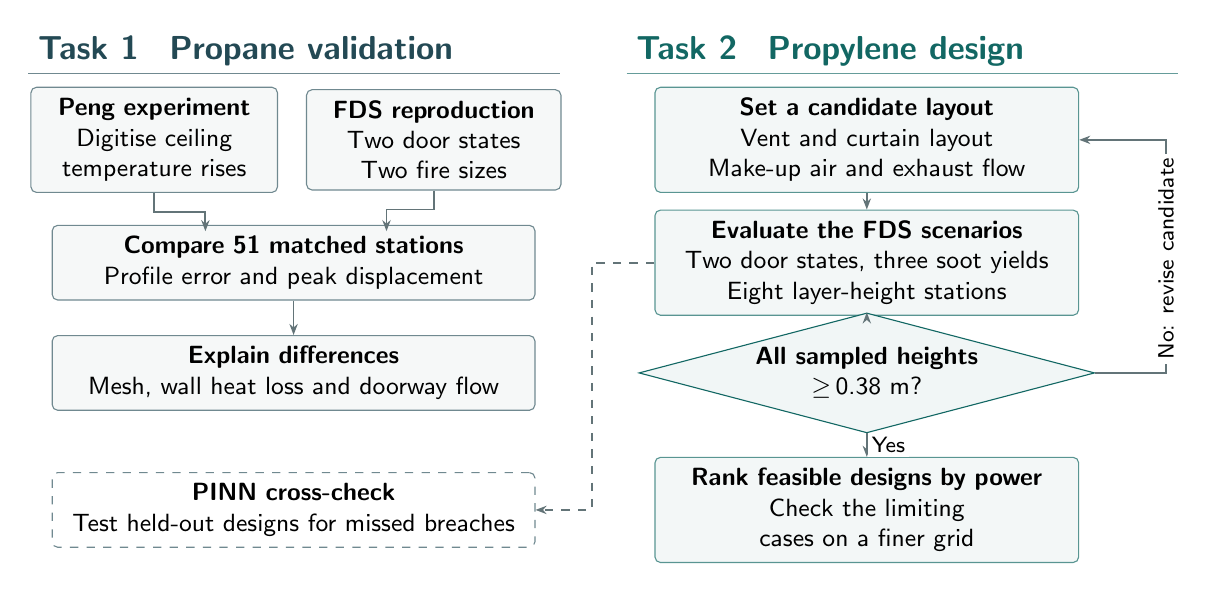
\begin{tikzpicture}[x=1cm,y=-1cm,font=\sffamily\small,
  head/.style={font=\sffamily\bfseries\large,anchor=west},
  box/.style={draw=navy!65,fill=navy!4,rounded corners=2pt,align=center,inner sep=4pt},
  design/.style={box,draw=teal!70,fill=teal!5},
  route/.style={draw=rulegray,line width=.65pt,-{Stealth[length=4pt]}},
  note/.style={font=\sffamily\footnotesize,fill=white,inner sep=1.5pt}]
\node[head,text=navy] at (0,0) {Task 1 \enspace Propane validation};
\node[head,text=teal] at (7.6,0) {Task 2 \enspace Propylene design};
\draw[navy!65] (0,.28)--(6.75,.28);
\draw[teal!65] (7.6,.28)--(14.6,.28);
\node[box,text width=2.85cm] (exp) at (1.60,1.12)
  {\textbf{Peng experiment}\\Digitise ceiling\\temperature rises};
\node[box,text width=2.95cm] (fds) at (5.15,1.12)
  {\textbf{FDS reproduction}\\Two door states\\Two fire sizes};
\node[box,text width=5.85cm] (compare) at (3.37,2.68)
  {\textbf{Compare 51 matched stations}\\Profile error and peak displacement};
\draw[route] (exp.south)--++(0,.24)-|(2.25,2.28);
\draw[route] (fds.south)--++(0,.24)-|(4.55,2.28);
\node[box,text width=5.85cm] (diagnose) at (3.37,4.08)
  {\textbf{Explain differences}\\Mesh, wall heat loss and doorway flow};
\draw[route] (compare.south)--(diagnose.north);
\node[design,text width=5.10cm] (layout) at (10.65,1.12)
  {\textbf{Set a candidate layout}\\Vent and curtain layout\\Make-up air and exhaust flow};
\node[design,text width=5.10cm] (measure) at (10.65,2.68)
  {\textbf{Evaluate the FDS scenarios}\\Two door states, three soot yields\\Eight layer-height stations};
\draw[route] (layout.south)--(measure.north);
\node[diamond,aspect=3.8,draw=teal,fill=teal!6,align=center,inner sep=1.4pt] (decision) at (10.65,4.08)
  {\textbf{All sampled heights}\\$\geq$\,0.38 m?};
\draw[route] (measure.south)--(decision.north);
\draw[route] (decision.east)--(14.45,4.08)--(14.45,1.12)--(layout.east);
\node[note,rotate=90] at (14.45,2.63) {No: revise candidate};
\node[design,text width=5.10cm] (select) at (10.65,5.82)
  {\textbf{Rank feasible designs by power}\\Check the limiting cases on a finer grid};
\draw[route] (decision.south)--node[right,note]{Yes}(select.north);
\node[box,dashed,fill=white,text width=5.85cm] (pinn) at (3.37,5.82)
  {\textbf{PINN cross-check}\\Test held-out designs for missed breaches};
\draw[route,dashed] (measure.west)--(7.16,2.68)--(7.16,5.82)--(pinn.east);
\end{tikzpicture}
\end{document}
